\documentclass[11pt]{article}
\usepackage[utf8]{inputenc}
\usepackage[russian,english]{babel}
\usepackage[T2A,T1]{fontenc}
\usepackage[linewidth=1pt]{mdframed}
\usepackage[a4paper, 
   left=25mm,
   right=25mm,
   top=25mm,
   bottom=25mm]{geometry}
\usepackage{amsmath,amsthm,amssymb}
\usepackage{lipsum}
\usepackage{lmodern}
\usepackage{tcolorbox}
\usepackage{hyperref}
\usepackage{relsize}
\usepackage{array}
\usepackage{enumitem}
\usepackage{graphicx}
\usepackage{float}
\usepackage{hyperref}
\usepackage{pythontex}
\usepackage{apacite}
\usepackage{lscape}
\usepackage{listings}
\usepackage{setspace}
\usepackage{fancyhdr,etoolbox}
\usepackage{float}
\usepackage{rotating}
\pagestyle{fancy}
\linespread{1.25}

\newtheorem{theorem}{Theorem}

\newcommand\myarray[1]{%
  \begingroup
  \renewcommand\arraystretch{1}
  \left\{\begin{array}{@{}l@{}} #1 \end{array} \right.
  \endgroup}
  
\fancyhead[LE,RO]{\nouppercase{\slshape }}
\fancyhead[LO,RE]{\nouppercase{\slshape \leftmark}}
\fancyfoot[C]{\thepage}

\title{
\vspace{-1cm}
\includegraphics[width=1.4in]{Images/HSE_Logo.eps}\\
\vspace{2cm}
\normalsize{\textsc{Thesis}}\\ \vspace{0.5cm}
\LARGE{\textbf{Comparative analysis of the option pricing methods}}
\vspace{3.5cm}}

\author{
\large{Author}: \Large{Dmitrii Kim}\\
\large{Supervisor}: \Large{Ivan Kolesnikov}\\
		\vspace{3.0cm} \\
		International College of Economics and Finance\\
  \textbf{National Research University Higher School of Economics}\\
  Moscow, Russia
  \vspace{0.8cm}
  } \date{Moscow, 2022}
%______________________________________________________________________________
\begin{document}
%Russian title
\thispagestyle{plain}
\begin{otherlanguage*}{russian}
\begin{center}
\Large{ФЕДЕРАЛЬНОЕ ГОСУДАРСТВЕННОЕ АВТОНОМНОЕ \\
ОБРАЗОВАТЕЛЬНОЕ УЧРЕЖДЕНИЕ ВЫСШЕГО ОБРАЗОВАНИЯ \\
«НАЦИОНАЛЬНЫЙ ИССЛЕДОВАТЕЛЬСКИЙ УНИВЕРСИТЕТ \\
«ВЫСШАЯ ШКОЛА ЭКОНОМИКИ»}\\
\vspace{0.3cm}
\Large{\textbf{Международный институт экономики и финансов}}\\
\vspace{0.7cm}
\Large{Ким Дмитрий Алексеевич\\}
\vspace{0.3cm}
%\textbf{Сравнительный анализ методов оценки опционов}\
\textbf{СРАВНИТЕЛЬНЫЙ АНАЛИЗ МЕТОДОВ\\ ОЦЕНКИ ОПЦИОНОВ\\
\vspace{7pt}
%\large{(Comparative analysis of the option pricing methods)}}\\
\large{(COMPARATIVE ANALYSIS OF THE OPTION PRICING METHODS)}}\\
\vspace{0.2cm}
Курсовая работа\\
\vspace{3pt}
БАКАЛАВРСКАЯ РАБОТА\\
\vspace{3pt}
по направлению подготовки 38.03.01 «Экономика»\\
\vspace{3pt}
образовательная программа «\textbf{Программа двух дипломов по \\ экономике НИУ ВШЭ и Лондонского университета}»
\vspace{1.5cm}

\begin{flushright}
\large{Научный руководитель:\\
\noindent\rule{4.5cm}{0.4pt}\\
И.А. Колесников\\}
\end{flushright}

\vfill
Москва, 2022
\end{center}
\end{otherlanguage*}


%table of contents
\newpage
\thispagestyle{plain}
\tableofcontents
\newpage
%______________________________________________________________________________
\section{Introduction}
\par Economic news frequently discusses the significant losses that traders in the financial derivatives market have sustained. The financial world was shocked when major firms apparently lost hundreds of millions, if not billions, of dollars. Due to these catastrophes, several well-known institutions have failed. Often while these stories are important, fascinating, and even surprising, they have hurt the reputation of using derivatives. However, when used appropriately, they are essential tools for effective risk management, therefore a strong evaluation strategy is necessary.
\par The goal of this work is to explain what is option, what types of options are there, also to give mathematical reasoning to the famous methods of determination of the option's price, and to show how they could be used with modern programming language.
%______________________________________________________________________________
\section{Literature and learning material review}
\begin{itemize}
    \item Breakthrough work which defined further development of derivative pricing and risk management. Black-Scholes formula provides a unique theoretical price for European options. \cite{B_S_73}
    \item Formalized Binomial tree approach for modeling the option price. \cite{C_R_R_79}
    \item Valuing American Options by estimating conditional expected payoff via Least-Squares. \cite{L_S_01}
    \item University of London Study guide. Fundamental financial theory. \cite{UoL}
    \item Book on derivatives for graduate and advanced undergraduate courses in business, economics, and financial engineering.  \cite{Hull_9}
    \item A series of internet blog posts about the Binomial Option Pricing Model with implementation in Python programming language \cite{JT_1, JT_2, JT_3, JT_4}
    \item An overview of the most common Machine Learning techniques applied to pricing European call options. \cite{C_21}
    \item Series of the lectures presented by industry professionals "on mathematical foundations of modeling in finance with those focused on important real-world problems" \cite{MIT}
    \item Advanced undergraduate course for \cite{ICEF_A} \\
Other articles: \cite{M_73}, \cite{M_76}, \cite{C_R_76}, \cite{B_76}, \cite{H_W_87}, \cite{B_C_C_97}, \cite{H_P_81}
\end{itemize}

\newpage
%______________________________________________________________________________
\section{Theoretical background}
\newtheorem{definition}{Definition}
\begin{definition}
Financial derivatives \\ Financial instruments which depend on the value of another assets.
\end{definition}
"Financial derivatives are financial instruments that are linked to a specific financial instrument or indicator or commodity, and through which specific financial risks can be traded in financial markets in their own right." \cite{IMF}

\begin{definition}
Derivative security (contingent claim) \\ An agreement between a buyer and a seller.
\end{definition}

As derivatives dependent upon the price of asset (usually stock), then in order to determine the present value, one has to know the payoffs schedule, as well as the stock's possible trajectories. The latter is a subject of modeling, bringing the assumptions on the type and characteristics of asset's behavior. Typically, the main division comes from assuming discrete or continuous behavior. 

\newpage
\subsection{Options}
\subsubsection{Definition}
Option is a contingent claim that gives one investor, holding the long position, the option (but not the obligation) to buy/sell an underlying asset 
\[\begin{tabular}{ | m{3.5cm}| m{3.2cm} |  m{3.2cm} |} 
  \hline
  Options | Position & Long & Short\\ 
  \hline
  Call & option to buy & must agree to sell\\ 
  \hline
  Put & option to sell & must agree to buy\\ 
  \hline
\end{tabular}\]
for a specified at the time of singing a contract price (strike price) \cite{JT_1}

\[\begin{tabular}{ | m{2cm}| m{7cm} |} 
  \hline
  European & at specified future time (expiration time)\\ 
  \hline
  American & at any date before the expiration time\\ 
  \hline
\end{tabular}\]

One may plot the return of the option in Stock price - Profit/Loss plane:
\begin{figure}[H]
  \centering
  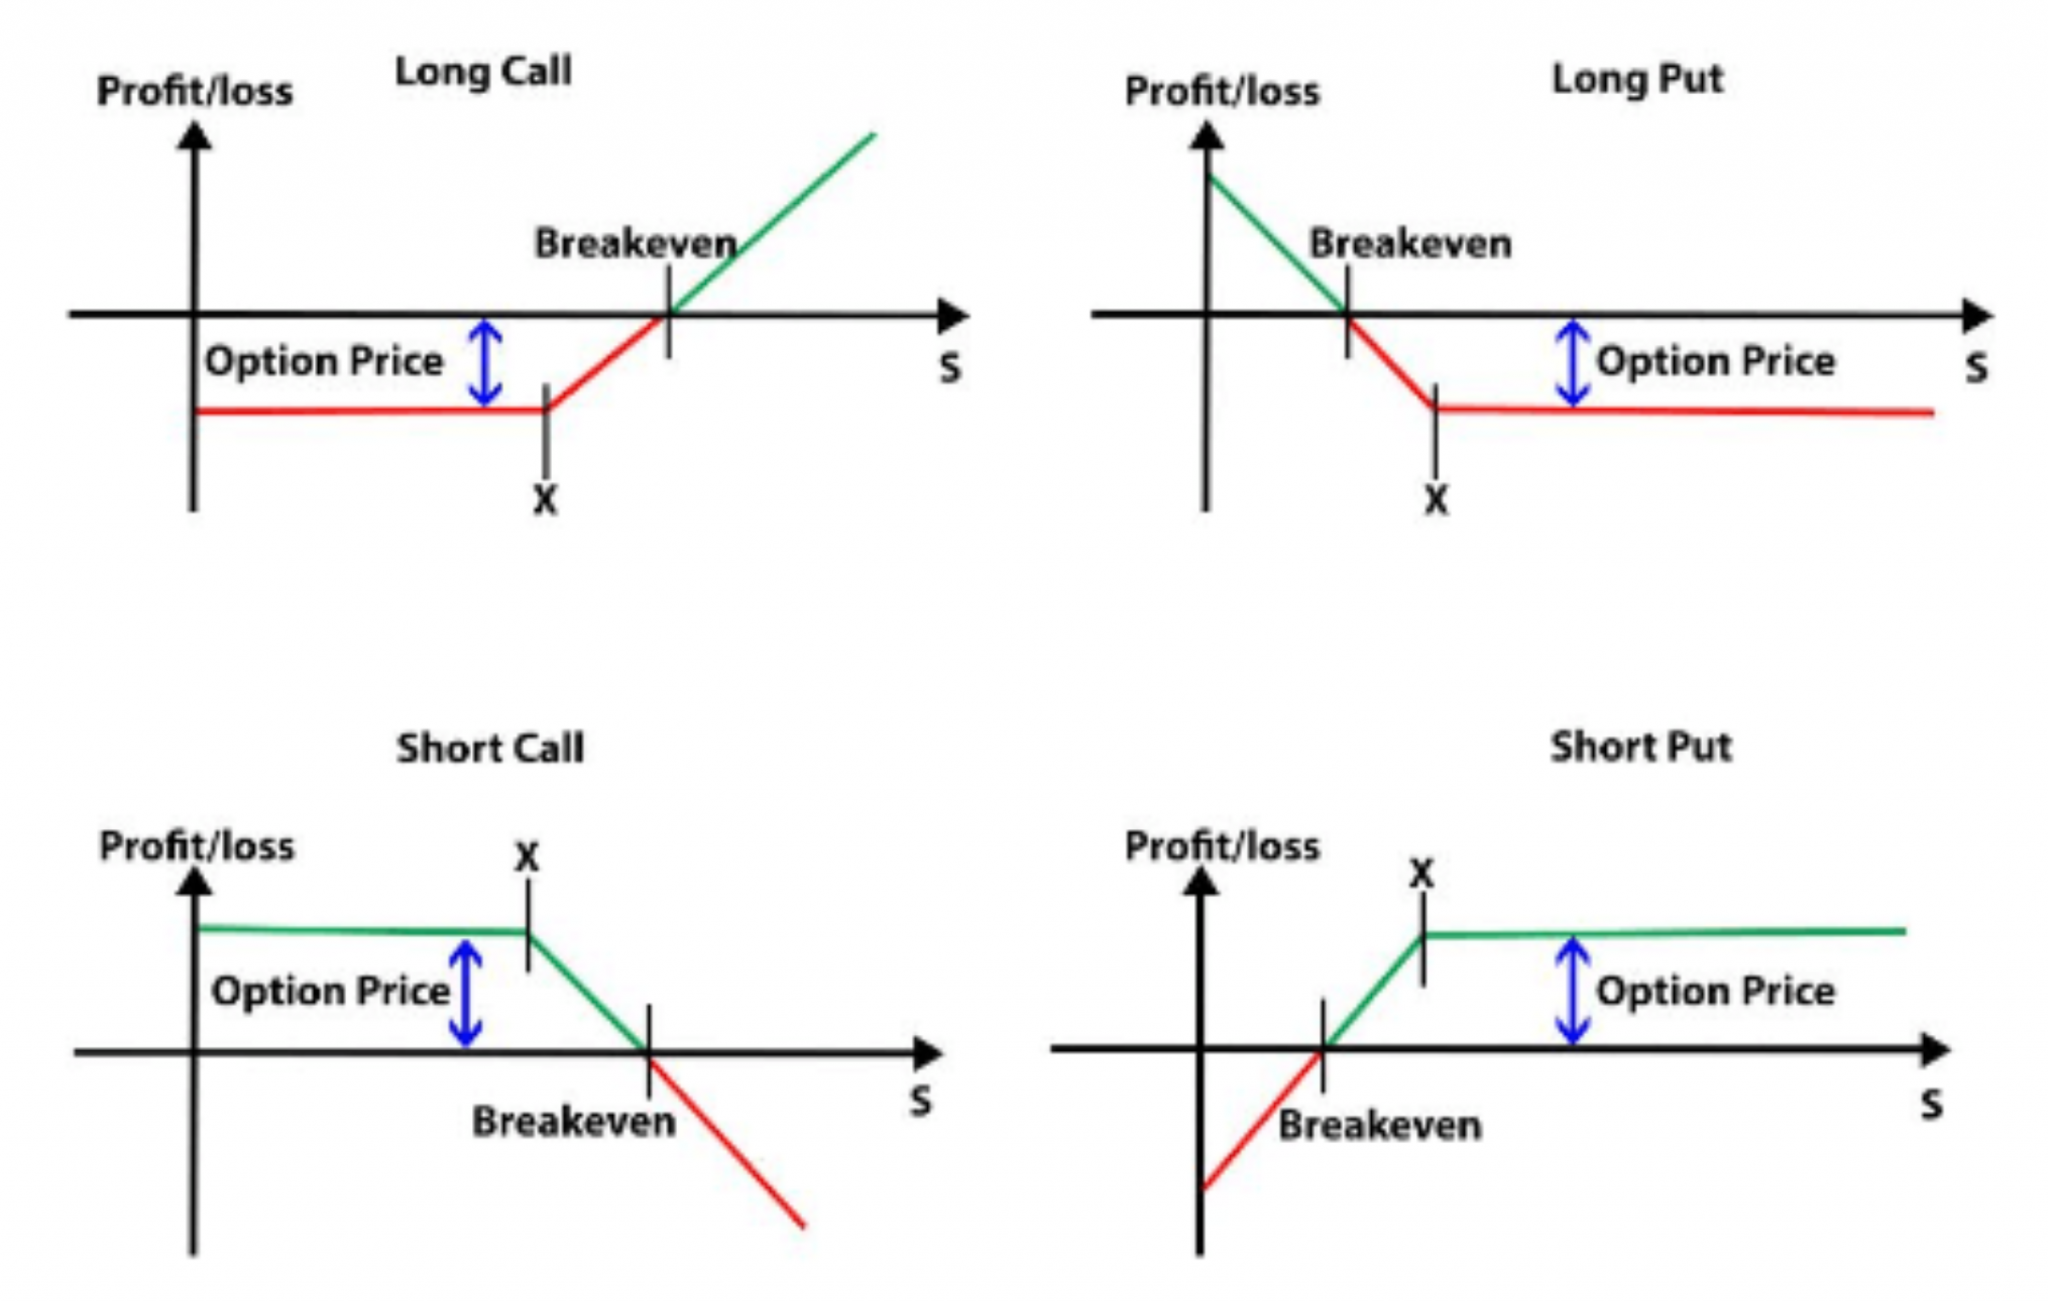
\includegraphics[scale=0.2]{Term paper/Images/PAYOFF.png}
  \caption{Payoffs for European Call and Put options \protect\cite{payoffs}}
  \label{fig:payoff}
\end{figure}


\textbf{Why to own an option?}   It is cheaper than holding the asset itself, as well as decreases the downside risk of the investment.  
Also used as an insurance to hedge risk. For example, if investor has the stock, he may buy a put option to save the value of his asset. 
Note that the short position has \textbf{no limit} for the losses! 

\newpage
\subsubsection{The Simplest Binomial Model (One period, one risky asset, two states)}
\label{sec:sbin}
Consider the following characteristics of an \textbf{European call option}:
\[\begin{tabular}{ | m{5cm}| m{3.2cm} | } 
  \hline
  Stock price today ($t=0$) & $S_0 = 100£$ \\ 
  \hline
  Stock price in 1 year ($t=1$) & $S_L = 80£$ (Low), $S_H = 120£$ (High)\\ 
  \hline
  \textit{Strike price} & $K = 100£$ \\ 
  \hline
\end{tabular}\]
What is fair price of the option $C_0^K$?\\
Profit at $t=1$ (Payoff schedule):
\[
C_1^K = (S_1-K)^+ := \max{(S_1-K, 0)} = 
\begin{cases}
S_1-K & \mbox{if } S_1 > K\\
0 & \mbox{if } S_1 \leqslant  K\\
\end{cases} \\
\]
Where $S_T$ - price of 1 share, $C_T^K$ - value of the Call option with strike price $K$ at $t=T$.\\ 
It is reasonable to assume the \textbf{no-arbitrage condition}: \[\textit{Portfolios with the same cash flows are identical in value.}\]
From it naturally comes \textbf{pricing by replication}: create a portfolio: $\vec{H} = (H_0, H_1) = (b,a)$ - investments at $t=0$, where $a$\footnote{Number of shares $a$ is not always integer. Increasing the number of shares solves the problem.} 
amount of shares and $b$£ in cash.\footnote{Negative values represent short selling ($a < 0$) or borrowing ($b < 0$).}\\
Value of the portfolio: $V_t(\vec{H}) = P(S_t) = aS_t + b$ and we know that
\[
P(80£) = 0£ \text{ and } P(120£) = 20£ => a = 1/2 \text{ and } b = -40£ \footnote{Cash $b$ is negative. Solved by an obligation to make a payment. (ex. take a loan, write a bond)}
\]
We replicated the option's payoff in 1 year with a portfolio by buying a half of the underlying stock and borrowing 40£. So, the price of the portfolio today is $P(100£)= 1/2 * 100£ - 40£ = 10£$. And by the `no-arbitrage principle` the price of an option is equal to it $C_0^K = V_0(\vec{H}) = 10£$.\\

In general, we know: $S_L \leq S_0 \leq S_H$, $P(S_1) = C_1^K$ \\
\[\myarray{P(S_L) = {C_1^K}_H = 0\\P(S_H) = {C_1^K}_L = S_H - S_0 \geq 0}
\Rightarrow
\myarray{aS_L + b  =  0)\\aS_H + b  =  S_H - S_0 }
\Rightarrow
\myarray{a = \frac{S_H - S_0}{S_H - S_L}\\b = - a*S_1}\]
\[\text{Then, } V_0(\vec{H}) = P(S_0) = aS_0 + b = \frac{S_H - S_0}{S_H - S_L}*S_0 + - a*S_1 = \underline{\frac{(S_H - S_0)(S_0 - S_L)}{S_H - S_L} = C_0^K}.\]

\newpage
\subsubsection{Risk-Neutral Pricing:}
Let us now implement probabilities into our model: $S_0 > 0$, $S_H > S_L > 0$, $p \in [0,1]$
\[t=1: S_1 = \begin{cases} S_H, & \mbox{if $\omega_H$}\\ S_L, & \mbox{if $\omega_L$} \end{cases} \text{  } C_1^K = \begin{cases} S_H-S_0, & \mbox{if p}\\ S_H-S_0, & \mbox{if 1-p} \end{cases}\]
Two states of the world at $t=1$: $\omega_H$ and $\omega_L$ $\Rightarrow$ 
\\The probability space: $\Omega =\{\omega_H, \omega_L\}$, $P(\omega_H)=p$ and $P(\omega_L)=1-p$\\
The buyer pays $C_0^K$ (non-random) at $t=0$, and earns $C_1^K(w)$ (random) at $t=1$ \\The conditions when cash is paid at each situation are fixed in the contract $\{C_1^K(\omega_H), C_1^K(\omega_L)\}$\\

\textbf{Question}: Given $C_1^K(W)$, what is fair price $C_0^K$?\\
If we ignore time value of money (interest rates), then the expected value of option in the future should be equal to the current value of it:\\
\[C_0^K = \mathbb{E}{[C_1^K]}\]
Then expected value of the option in the next year:
\[\mathbb{E}{[C_1^K]} = (S_H - S_0)*p + 0 * (1-p) = \underline{(S_H - S_0)p = C_0^K} \text{ - depends on $p$}\]

\textbf{Risk-Neutral probability}\\
In order to price the option, we need to find the probability of exercising the option. Using risk-neutrality concept, investor ignores the riskiness of the stock price:
\[\begin{cases} S_0 = E(S_1) \\ E(S_1) = S_H*p + S_L*(1-p) = S_L + (S_H - S_L)p \end{cases} \Rightarrow S_0 = S_L + (S_H - S_L)p \]
\[\Rightarrow p =  \frac{S_0 - S_L}{S_H - S_L} \textit{ - risk-neutral probability}\]
\[C_0^K = (S_H - S_0) * p = \frac{(S_H - S_0)(S_0 - S_L)}{S_H - S_L}\text{ same as in the replication approach!}\]
\[\text{Now, let } q_H = \frac{S_0 - S_L}{S_H - S_L} \text{ and } q_L = \frac{S_H - S_L}{S_H - S_L} 
\Rightarrow q_H > 0, q_L > 0 \text{ and } q_H + q_L = 1  \cite{ICEF}\] 
\[\Rightarrow V_0(\vec{H})= {C_1^K}(\omega_H)*q_H + {C_1^K}(\omega_L)*q_L = \mathbb{E^Q}{[C_1^K]} \text{  with a new \textbf{risk-neutral probability measure }}Q \footnote{$Q$ on $\Omega =\{\omega_H, \omega_L\}$:, $Q(\omega_H)=q_H$ and $(Q\omega_L)=q_L$}\]

In reality, $value$ $today < expected$ $future$ $value$ for any stock, because the future value is\\ uncertain and one can just keep the current asset and not take any risk.\\
Note that with the risk-neutral probability measure $Q$, the price of the option $C_0^K$ does not depend upon the probability of the $\omega_H$, meaning that the price is free of probability. 

\newpage
\subsection{Option Pricing methods}
There are many option pricing methods, they are different in the used assumptions such as a type of behavior of the underlying stock (ex. discrete (Random Walk), or continuous (Geometric Brownian Motion)). Most of them are based on the \textit{risk-neutrality principle}. The most used ones are:
\begin{itemize}
    \item Binomial/Trinomial Tree
    \item Black-Scholes model
    \item Monte Carlo simulation
    \item Finite difference methods
\end{itemize}
The list is not exhaustive, however it covers common techniques used both in Academia and Industry. This paper dives deep into the \textit{Binomial tree} model, and touches the \textit{Black-Scholes} model.

\subsubsection{Binomial Tree}
\label{bintree}
This method was first formalized in the article "Option Pricing: A Simplified Approach" by \cite{C_R_R_79}.\\
\textbf{Idea - Random Walk}: Divide the life of the option into small time intervals $\Delta{t}$.\\
Assume that at each time the price $S$ of the underlying stock at the beginning of the interval either goes 'up' to $Su$ with probability $p$, or 'down' $Sd$ with probability $1-p$\\ 

\begin{figure}[H]
  \centering
  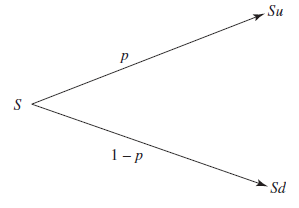
\includegraphics[scale=1]{Term paper/Images/bin_tree.PNG}
  \caption{Paths for asset price movement in $\Delta{t}$ under the binomial model \protect\cite{Hull_9}}
  \label{fig:bin_tree}
\end{figure}

As division, i.e. the number of time steps goes to infinity, Binomial tree model converges to the Black-Scholes-Merton model. Showing that discrete behaviour in the limit becomes continuous. \footnote{proof why is that true}

\newpage
\textbf{Risk-Neutral Valuation principle}\\
The principle states that the value of a derivative can be measured under the assumption that the world is risk neutral.
\begin{itemize}
    \item Assume $\mathbb{E^Q}{[r_i]} = r_f$ for any asset $A_i$.\\ Where $r_i$ - return of the asset, $r_f$ - risk-free rate, $Q$ - risk-neutral measure.
    \item Value of the derivative's payoff is equal to discounted at the risk-free interest rate the expected value: $V_0 = df(t) * \mathbb{E^Q}{[X]}$, where $df(t)$ discount factor after period $t$,
\end{itemize}
\[
df(t) = \begin{cases} e^{-rt} & \mbox{if continuous compounding}\\ 
(1+r)^{-t} & \mbox{if discrete} \end{cases}
\]  
Continuous compounding will be used. \footnote{As $n\to\infty$, discrete compounding $\to$ continuous one: $\lim_{n\to\infty} (1+\frac{r}{n})^{nt} = e^{rt}$}\\

\textbf{Determination $p$, $u$, and $d$}
%Denote yield of an option as $q$, and risk-free interest rate as $r$. 
\begin{equation}
\label{eqn:param}
\text{Parameters of the model}: S_0 > 0, u > 1, 1 > d \geqslant 0, 1 \geqslant p \geqslant 0, \Delta{t} > 0, n > 0, r > 0
\end{equation}

Let us fix the \hyperref[sec:sbin]{model} defined above by changing some of the parameters: $ S_H = S_0*u; S_L = S_0*d$. Where $(u - 1)*100\%$ and $(d - 1)*100\%$ are stocks percentage change in both directions.\\
Furthermore, by adding interest rates into the model we get new risk-neutral probability:
\[S_0 = df(\Delta{t})*\mathbb{E}{S_1} \Rightarrow p = \frac{\mathbb{E}{S_1} - S_L}{S_H - S_L} = \frac{S_0/df(\Delta{t})- S_0d}{S_0u - S_0d} \Rightarrow\]
\[Q(\omega_H) = q_H = \frac{e^{r\Delta{t}} - d}{u - d} \text{ and } Q(\omega_L) = q_L = \frac{u - e^{r\Delta{t}}}{u - d}\]
Knowing that $C_1^K = (S_1-K)^+$, use the risk-neutral valuation principle to price the option
\[C_0^K = df(t) * \mathbb{E^Q}{[C_1^K]} = e^{-r\Delta{t}}[{C_1^K}(\omega_H)*q_H + {C_1^K}(\omega_L)*q_L]\]
\begin{equation}
\label{eqn:price}
C_0^K = e^{-r\Delta{t}}({S_0u - K})\frac{e^{r\Delta{t}} - d}{u - d} 
\end{equation}
Let's check the consistency of the model: $S_0 = 100£$, $u = 1.2$, $ d = 0.8$, $r = 0\%$, $\Delta{t} = 1$.
\[C_0^K = e^{-0*1}({100*1.2 - 100})\frac{e^{0*1} - 0.8}{1.2 - 0.8} = 20 * \frac{0.2}{0.4} = 10£\]\label{task}
As expected, the formula (\ref{eqn:price}) gave the same result. Now add risk-free interest rate $r = 5\%$.
\[C_0^K = e^{-0.05*1}({100*1.2 - 100})\frac{e^{0.05*1} - 0.8}{1.2 - 0.8} = 0.951*20 * \frac{1.051 - 0.8}{0.4} = 19.02 * \frac{0.251}{0.4} = 11.94£\]
The price increased, meaning positive relationship between the price of the call option $C_0^K$ and the risk-free interest rate $r$. The intuition is that the strike price $K$ in the future is decreasing in its present value with increasing interest rate.


\newpage
\textbf{Generalize: proof by \cite{ICEF_A}}
\begin{figure}[H]
  \centering
  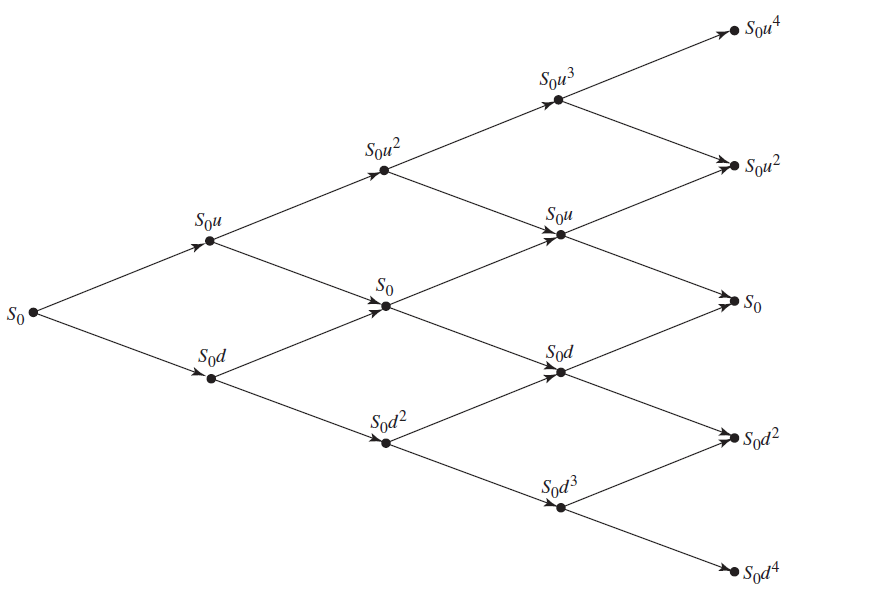
\includegraphics[scale=0.7]{Term paper/Images/big_tree.png}
  \caption{The tree with 4 time intervals \protect\cite{Hull_9}}
  \label{fig:btree}
\end{figure}
The stock price $S_n$ after $n$ time intervals is a random variable. Denote the change after $k$ time interval $X_k$. It is also a random variable. 

\[\begin{tabular}{ | m{0.5cm}| m{0.5cm} | m{0.6cm} |} 
  \hline
  $X_k$ & u & d \\
  \hline
  P & p & 1-p \\ 
  \hline
\end{tabular}
\hspace{0.5cm} \text{where } p = \frac{e^{r\Delta{t}} - d}{u - d} \in [0,1]\]
Because $X_1,...,X_n$ are independent and identically distributed (i.i.d.), then one may see that 
\[S_n = S_0X_1...X_n = S_0*u^Y*d^{n-Y}\]
\[Y \sim Binom(n,p) \Rightarrow P(Y=k) = C_n^kp^k(1-p)^{n-k}, \text{ } k = 0,...,n\]
Where random variable $Y$ is a number of "up" movements. It is distributed as $Binomial$ with number of tries $n$ and probability of success.

\textbf{The option price derivation:}
As was already stated the current value of the option, i.e. the option price is a discounted expected payoff under the risk-neutral measure. Assumed stock price movement allow us to calculate the price analytically. $t = n*\Delta{t}$
\[C_0^K = df(t) * \mathbb{E^Q}{[C_1^K]} =  e^{-rn\Delta{t}}*\mathbb{E^Q}{(S_n-K)^+} = e^{-rn\Delta{t}}\mathlarger{\sum}_{k=1}^{n} (S_0u^kd^{n-k} - K)^+P(Y=k) = \]
\[ = e^{-rn\Delta{t}}\mathlarger{\sum}_{k=1}^{n} (S_0u^kd^{n-k} - K)^+C_n^kp^k(1-p)^{n-k}\]
\newpage
Because $(S_0u^kd^{n-k}-K)^+ = 0$ when $S_0u^kd^{n-k} < K$.\footnote{$S_0u^kd^{n-k} = S_0d^n(\frac{u}{d})^k < K \Leftrightarrow (\frac{u}{d})^k < \frac{K}{S_0d^n} \Leftrightarrow 
k\ln{\frac{u}{d}} < \ln{\frac{K}{S_0d^n}} \Leftrightarrow  k < \frac{\ln{(\frac{K}{S_0d^n})}}{\ln{(\frac{u}{d})}}$}
\[
(S_0u^kd^{n-k}-K)^+ > 0 \text{ for $k \geqslant a$, where }  a = \left\lceil \mathlarger{\frac{\ln{(\frac{K}{S_0d^n})}}{\ln{(\frac{u}{d})}}} \right\rceil
\]
Where $\lceil x \rceil$ is the ceiling function, i.e. smallest integer greater than or equal than $x$.\\Now continue the derivation process:
\[C_0^K = e^{-rn\Delta{t}}\mathlarger{\sum}_{k=1}^{n} (S_0u^kd^{n-k} - K)^+C_n^kp^k(1-p)^{n-k} = e^{-rn\Delta{t}}\mathlarger{\sum}_{k=a}^{n} (S_0u^kd^{n-k} - K)C_n^kp^k(1-p)^{n-k} = \]
\[ = \frac{S_0}{e^{n\Delta{t}}}\mathlarger{\sum}_{k=a}^{n} C_n^k(up)^k((1-p)d)^{n-k} - \frac{K}{e^{n\Delta{t}}}\mathlarger{\sum}_{k=a}^{n} C_n^kp^k(1-p)^{n-k}\]
Now denote $\mathlarger{p' = up*e^{-n\Delta{t}} > 0}$ to make new probability measure, then check that sum is equal to one.
\[
\frac{up}{e^{n\Delta{t}}} + \frac{(1-p)d}{e^{n\Delta{t}}} = \frac{p(u-d) + d}{e^{n\Delta{t}}} =  \frac{[(e^{r\Delta{t}} - d)/(u - d)]*(u-d) + d}{e^{n\Delta{t}}} = \frac{e^{n\Delta{t}}}{e^{n\Delta{t}}} = 1
\]
So, $\mathlarger{\frac{(1-p)d}{e^{n\Delta{t}}} = 1 - p'}$ this allows us to define a new random variable $Y' \sim Binomial(n,p')$ and finish the formula for the price of European call option:
\[
C_0^K = S_0\mathlarger{\sum}_{k=a}^{n} C_n^k(p')^k(1-p')^{n-k} - \frac{K}{e^{n\Delta{t}}}\mathlarger{\sum}_{k=a}^{n} C_n^kp^k(1-p)^{n-k}=
S_0\mathlarger{\sum}_{k=a}^{n} P(Y' = k) - \frac{K}{e^{n\Delta{t}}}\mathlarger{\sum}_{k=a}^{n} P(Y = k) \Rightarrow
\]

\textbf{\underline{Cox-Ross-Rubinstein (CRR) formula}:} \cite{C_R_R_79}
\begin{equation}
\label{eqn:CRR}
\mathlarger{C_0^K = S_0*P(Y \geqslant a) - \frac{K}{e^{n\Delta{t}}}P(Y \geqslant a) = S_0\Phi[a;n,p] - Ke^{-n\Delta{t}}\Phi[a;n,p']}
\end{equation}

Where $\Phi[a;n,p]$ - a complementary $Binomial(n,p)$  distribution function,\\
\[a = \left\lceil \mathlarger{\frac{\ln{(\frac{K}{S_0d^n})}}{\ln{(\frac{u}{d})}}} \right\rceil \text{ if $a > n$, $C_0^K = 0$}\]
\[\mathlarger{p = \frac{e^{r\Delta{t}} - d}{u - d}}\text{, and } \mathlarger{p' = \frac{u}{e^{n\Delta{t}}}p}\]
Parameters of the model: $S_0 > 0, u > 1, 1 > d \in{(1,0]}, p \in{[0,1]}, \Delta{t} > 0, n > 0, r > 0$ \footnote{See the $u=1/d$ argument at \ref{u}}

\textbf{Note:}
As $n\to\infty$ CRR formula\ref{eqn:CRR} will converge to famous Black-Scholes formula for European call option.\cite{C_R_R_79} Indeed, the limiting case of $Binomial$ distribution by Central Limit theorem is $Normal$ distribution which is present in BS formula.\footnote{One may prove it both analytically and empirically} 
%______________________________________________________________________________
\newpage
\subsubsection{Black-Scholes model}
As opposed to the discrete nature of the Binomial tree model \ref{bintree}, the Nobel Prize winning model lies in the continuous space, using full apparatus of the Stochastic Calculus.\\
The key feature of the model is the stochastic differential equation which defines the stock price
\[
dS_t = \mu{S_t}dt + \sigma{S_t}dW_t \text{ \cite{B_S_73}} 
\]
The solution to the DE is random process $(S_t)_{t\geqslant0}$ distibuted as \textit{Geometric Brownian motion (GBM)}.\cite{S_73}
\[\mathlarger{S_t = S_0e^{(\mu-\frac{\sigma^2}{2})t+\sigma{W_t}},}\]
Where $\mu$ and $\sigma$ is the \textit{drift} and \textit{volatility}  of the stock per year,\\ 
$W_t$ is a \textit{Brownian motion}(or \textit{Wiener process}).

\begin{definition} \cite{ICEF_A} \\
\label{brownian}
Stochastic process $W = (W_t)_{t\geqslant0}$ is called \textit{Brownian motion} if
\begin{enumerate}
    \item $W_0 = 0$, $W_t - W_s \sim N(0, t-s)$ for any $t>s\geqslant0$
    \item {It is a process with \textit{independent increments}:\\ 
    $(W_{t_2} - W_{t_1})$, $(W_{t_4} - W_{t_3})$ - independent, for any $0 \leqslant t_1 < t_2$, $0 \leqslant t_3 < t_4$}
\end{enumerate}
\end{definition}

\begin{theorem}

\end{theorem}

The Black-Scholes formula allows us the calculate the price of European call and put options.
\begin{equation}
	\mathrm C(\mathrm S,\mathrm t)= \mathrm N(\mathrm d_1)\mathrm S - \mathrm N(\mathrm d_2) \mathrm K \mathrm e^{-rt}
	\label{eq:2}
\end{equation}
\[
	\mathrm d_1= \frac{1}{\sigma \sqrt{\mathrm t}} \left[\ln{\left(\frac{S}{K}\right)} + t\left(r + \frac{\sigma^2}{2} \right) \right] \text{, }
	\mathrm d_2= \frac{1}{\sigma \sqrt{\mathrm t}} \left[\ln{\left(\frac{S}{K}\right)} + t\left(r - \frac{\sigma^2}{2} \right) \right]
\]
\[
	N(x)=\frac{1}{\sqrt{2\pi}} \int_{-\infty}^{x} \mathrm e^{-\frac{1}{2}z^2} dz \text{  - c.d.f of standard normal distribution}
\]

The \textbf{derivation} of the formula requires solving \textit{Partial Differential Equations}. The \textit{Taylor} expansion in \textit{Ito Calculus} helps to solve it.\cite{ICEF_A} It comes as a surprise, but with not-trivial change of variables the underlying P.D.E. becomes the famous \textit{Heat Equation} which has been deeply studied by physicists. \footnote{}


%______________________________________________________________________________
\newpage
\section{Empirical estimation with Binomial Tree}
Let's implement in Python Binomial tree approach to value the European Call Option.

\begin{figure}[H]
  \centering
  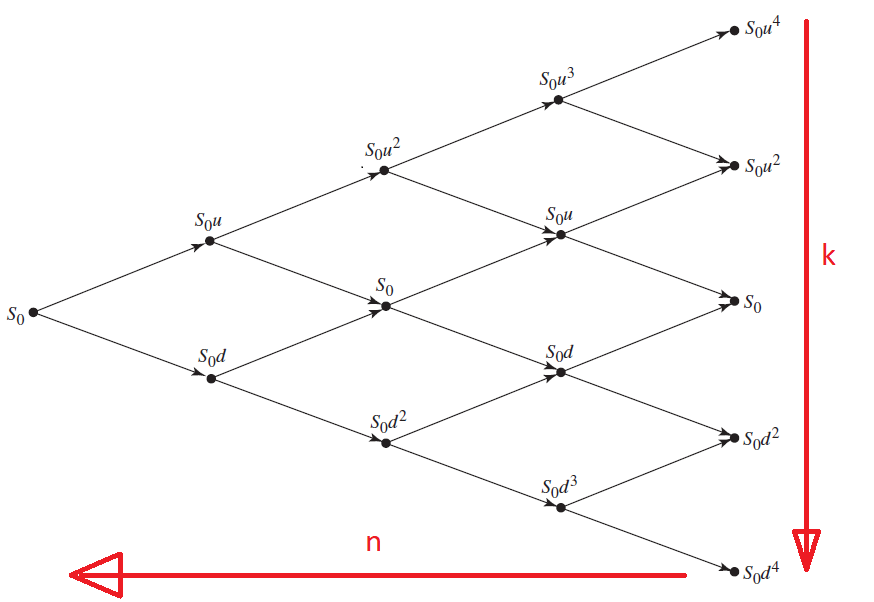
\includegraphics[scale=0.6]{Term paper/Images/tree_algo.png}
  \caption{Going through the tree with 4 time intervals}
  \label{fig:algtree}
\end{figure}
The algorithm stars evaluating option's value at last time interval $n=4$. For each state of the world (node) the value of option is its payoff $C_4^K(\omega_{u^k}) = max{(S_4(\omega_{u^k}-K), 0)}$, $k = -4,...,4$. Then it goes to depth of $n - 1 = 3$ intervals and at each node it evaluates the price. 

\noindent\begin{minipage}{0.44\textwidth}
Remark: $C_n^k \ne C_n^K$, $C_n^k$ - price of option at time interval $n$ with $k$ movements 'up'. \vspace{1cm}

$C_{n-1}^k = df(\Delta{t}) * \mathbb{E^Q}{[C_n^k]} =$ \\
$e^{-r\Delta{t}}[{C_4^{k+1}}(\omega_H)*p + {C_1^{k-1}}(\omega_L)(1-p)]$,\\
where $p$ - risk-neutral probability
\vspace{1cm}
\\ Repeat the process until $n = 0$: \\ \centerline{$C_0^K = C_0^0$}
\end{minipage}%
\hfill%
\begin{minipage}{0.7\textwidth}\raggedleft
\begin{figure}[H]
  \centering
  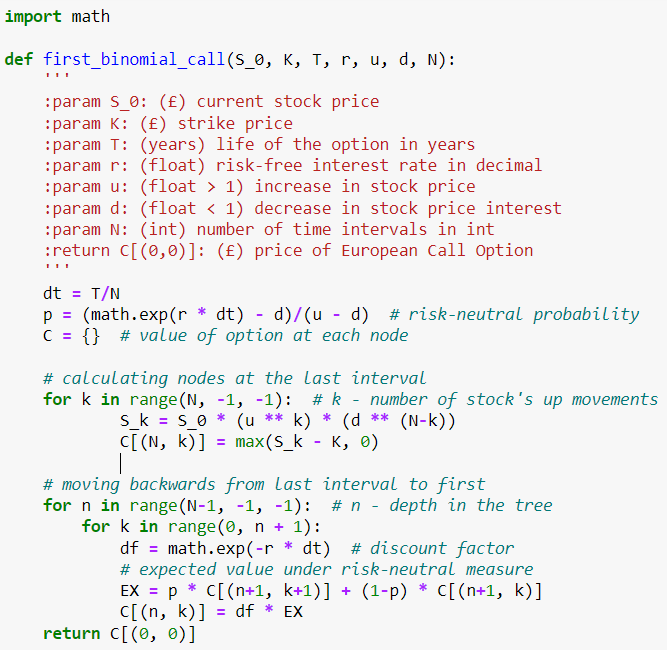
\includegraphics[scale=0.7]{Term paper/Images/first_bin_alg.PNG}
  \caption{Modified Python function for calculating the price of European Call option \protect\cite{JT_3}}
  \label{fig:fbinalg}
\end{figure}
\end{minipage}

\newpage
\textbf{Examples:}
Let's recalculate the prices from our task in \ref{task}
\begin{figure}[H]
  \centering
  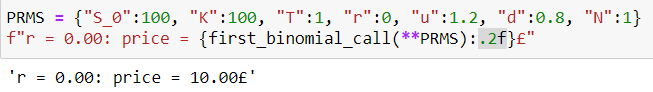
\includegraphics[scale=1]{Term paper/Images/output_1.PNG}
  \label{fig:out1}
\end{figure}

\begin{figure}[H]
  \centering
  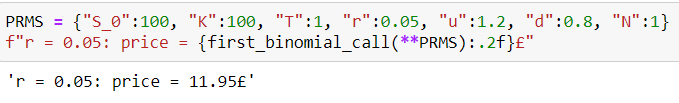
\includegraphics[scale=1]{Term paper/Images/output_2.PNG}
  \caption{Everything works as expected.}
  \label{fig:out2}
\end{figure}

\vspace{0.5cm}
\par What if we try to increase number of intervals $N$ keeping total time $T$ constant?
\begin{figure}[H]
  \centering
  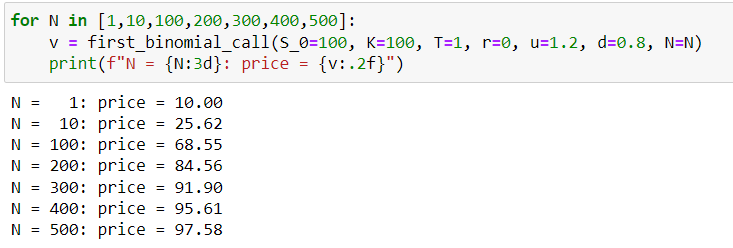
\includegraphics[scale=1]{Term paper/Images/output_3.PNG}
  \caption{As $N$ increases price seems to converge to the stock price. It is not wanted.}
  \label{fig:out3}
\end{figure}
The reason behind this behavior is the constant rate of change for a stock even for any, even really small, duration of the intervals. To make it more consistent with real world $u$ and $d$ should be changed.\\

\textbf{Choosing $u$ and $d$: Volatility}\\
\label{u}
An experienced statistician for any random variable (here $S_t$) would like to know its Expected value $\mathbb{E}{[S_t]}$ and Variance $\mathbb{V}{[S_t]} = \sigma^2$ . Standard deviation of a variable is a measure of volatility of an asset. The bigger 'up' $(u-1)$ or/and 'down' $(1-d)$ movements, the more volatile the stock is.
\par Typically the stock price is assumed to be distributed as \textit{Geometric Brownian motion (GBM)}.\cite{S_73}
\begin{equation}
\label{eqn:gbm}
\mathlarger{S_t = S_0e^{(\mu-\frac{\sigma^2}{2})t+\sigma{W_t}},}
\end{equation}
Where $\mu$ and $\sigma$ is the expected return and volatility (std.dev.) of the stock per year,\\ 
$W_t$ is a \textit{Brownian motion}\ref{brownian} (or \textit{Wiener process}).

\noindent The \textbf{percentage change} of the stock is distributed approximately Normal:
\begin{equation}
\label{eqn:dsdist}
\frac{\Delta{S}}{S} \sim N(\mu\Delta{t}, \sigma^2\Delta{t})
\end{equation}
Hence, its mean and variance are as follows:
\begin{equation}
\label{eqn:mv}
\mathbb{E}{[\frac{\Delta{S}}{S}]} = \mu\Delta{t} \text{ and } \mathbb{V}{[\frac{\Delta{S}}{S}]}= \sigma^2\Delta{t}
\end{equation}
By equating expected values and variances with \textit{Random Walk}, one finds the following relationships\footnote{Proof of the fact is in \cite{Hull_9} or \cite{FCS}}
\begin{equation}
\label{eqn:ud}
\mathlarger{u = e^{\sigma\sqrt{\Delta{t}}} \text{ and } d = \frac{1}{u}}
\end{equation}

\begin{figure}[H]
  \centering
  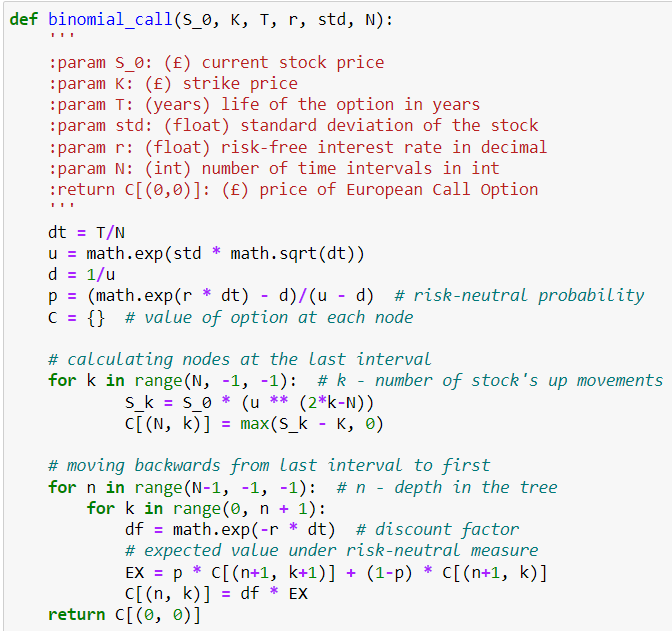
\includegraphics[scale=1]{Term paper/Images/bin_call.PNG}
  \caption{Final function for modelling with the Binomial Tree}
  \label{fig:bincall}
\end{figure}

\begin{figure}[H]
  \centering
  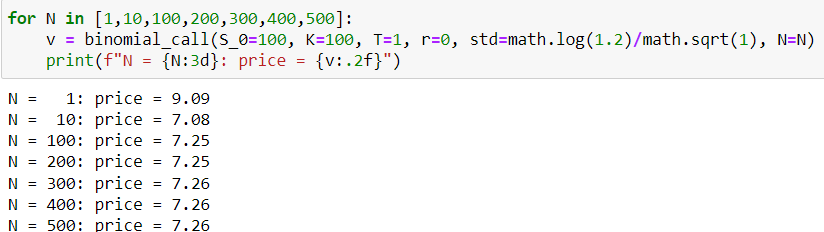
\includegraphics[scale=1]{Term paper/Images/output_4.PNG}
  \caption{consistent with the real-world results}
  \label{fig:out4}
\end{figure}

\begin{figure}[H]
  \centering
  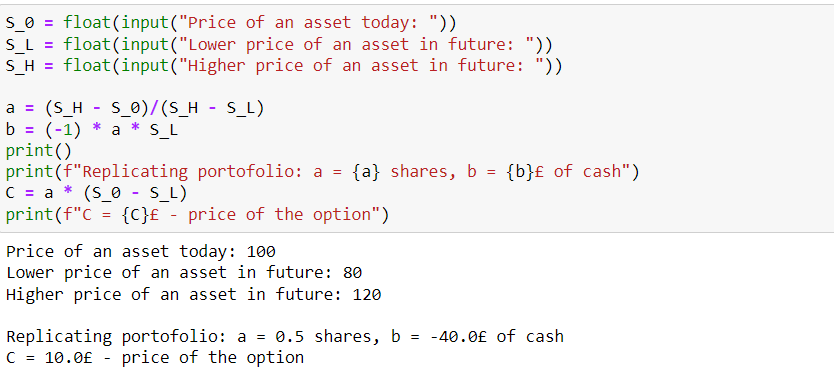
\includegraphics[scale=0.8]{Term paper/Images/simple_bin.PNG}
  \caption{Python code to the Simplest Binomial Model\protect\ref{sec:sbin}}
  \label{fig:out4}
\end{figure}
%______________________________________________________________________________
\vfill
\section{Conclusion}
\textbf{Discussion of the results:}
\par The thorough research was conducted, giving the understanding of options nature, as well as the 'state of the art' pricing methods. New branch of the financial mathematics was studied (stochastic, ito calculus) with the appropriate concepts such as (portfolio replication, risk-neutral probability measure, brownian motion, etc.). Implemented the valuation algorithms in Python programming language. Moreover, this article is written in \LaTeX, giving useful tool for further personal academical development.
\par Possible \textbf{further research} may focus on continuing the exploration of pricing models. For instance, visualizing the Wiener processes and estimating with it the prices, the Machine Learning regression analysis \cite{C_21}. Furthermore, the models should be tested on the real life data (MOEX, S\&P 500 and others). This will give deeper understanding on the applicability of the models.

%______________________________________________________________________________
\newpage
\bibliographystyle{apacite}
\bibliography{List_papers.bib} 
\end{document}
